% Figure 1: 3.5-bit Asymmetric Quantization Encoding Scheme
% This figure illustrates how two FP32 values are quantized and packed into 7 bits

\begin{figure}[t]
\centering

% Include TikZ for drawing
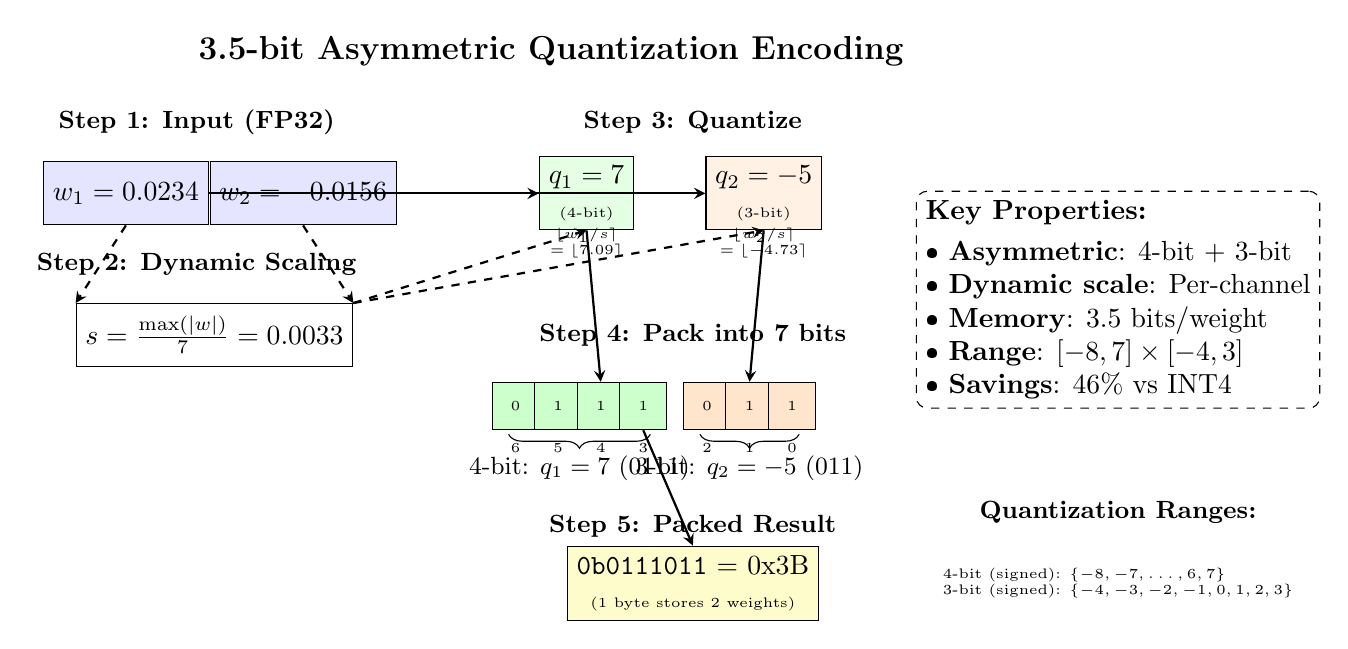
\begin{tikzpicture}[
    scale=0.9,
    box/.style={rectangle, draw, minimum width=1.2cm, minimum height=0.8cm, align=center},
    widerbox/.style={rectangle, draw, minimum width=2cm, minimum height=0.8cm, align=center},
    bitbox/.style={rectangle, draw, minimum width=0.6cm, minimum height=0.6cm, align=center, font=\tiny},
    arrow/.style={->, >=stealth, thick},
    label/.style={font=\small}
]

% Title
\node[font=\large\bfseries] at (0, 5.5) {3.5-bit Asymmetric Quantization Encoding};

%==============================================================================
% Step 1: Input FP32 values
%==============================================================================
\node[label] at (-5, 4.5) {\textbf{Step 1: Input (FP32)}};

\node[widerbox, fill=blue!10] (fp1) at (-6, 3.5) {$w_1 = 0.0234$};
\node[widerbox, fill=blue!10] (fp2) at (-3.5, 3.5) {$w_2 = -0.0156$};

%==============================================================================
% Step 2: Compute dynamic scale
%==============================================================================
\node[label] at (-5, 2.5) {\textbf{Step 2: Dynamic Scaling}};

\node[widerbox] (scale) at (-4.75, 1.5) {$s = \frac{\max(|w|)}{7} = 0.0033$};

% Arrows from inputs to scale
\draw[arrow, dashed] (fp1.south) -- (scale.north west);
\draw[arrow, dashed] (fp2.south) -- (scale.north east);

%==============================================================================
% Step 3: Quantize to integers
%==============================================================================
\node[label] at (2, 4.5) {\textbf{Step 3: Quantize}};

\node[box, fill=green!10] (q1) at (0.5, 3.5) {$q_1 = 7$\\{\tiny (4-bit)}};
\node[box, fill=orange!10] (q2) at (3, 3.5) {$q_2 = -5$\\{\tiny (3-bit)}};

% Quantization formulas
\node[font=\tiny, align=center] at (0.5, 2.8) {$\lfloor w_1 / s \rceil$\\$= \lfloor 7.09 \rceil$};
\node[font=\tiny, align=center] at (3, 2.8) {$\lfloor w_2 / s \rceil$\\$= \lfloor -4.73 \rceil$};

% Arrows
\draw[arrow] (fp1.east) -- (q1.west);
\draw[arrow] (fp2.east) -- (q2.west);
\draw[arrow, dashed] (scale.north east) -- (q1.south);
\draw[arrow, dashed] (scale.north east) -- (q2.south);

%==============================================================================
% Step 4: Bit packing (7 bits total)
%==============================================================================
\node[label] at (2, 1.5) {\textbf{Step 4: Pack into 7 bits}};

% Show bit layout
\node[bitbox, fill=green!20] (b6) at (-0.5, 0.5) {0};
\node[bitbox, fill=green!20] (b5) at (0.1, 0.5) {1};
\node[bitbox, fill=green!20] (b4) at (0.7, 0.5) {1};
\node[bitbox, fill=green!20] (b3) at (1.3, 0.5) {1};
\node[bitbox, fill=orange!20] (b2) at (2.2, 0.5) {0};
\node[bitbox, fill=orange!20] (b1) at (2.8, 0.5) {1};
\node[bitbox, fill=orange!20] (b0) at (3.4, 0.5) {1};

% Bit labels
\node[font=\tiny] at (b6.south) [below=0.05cm] {6};
\node[font=\tiny] at (b5.south) [below=0.05cm] {5};
\node[font=\tiny] at (b4.south) [below=0.05cm] {4};
\node[font=\tiny] at (b3.south) [below=0.05cm] {3};
\node[font=\tiny] at (b2.south) [below=0.05cm] {2};
\node[font=\tiny] at (b1.south) [below=0.05cm] {1};
\node[font=\tiny] at (b0.south) [below=0.05cm] {0};

% Bracket annotations
\draw[decorate, decoration={brace, amplitude=5pt, mirror}]
    (-0.6, 0.1) -- (1.4, 0.1)
    node[midway, below=0.15cm, font=\small] {4-bit: $q_1=7$ (0111)};

\draw[decorate, decoration={brace, amplitude=5pt, mirror}]
    (2.1, 0.1) -- (3.5, 0.1)
    node[midway, below=0.15cm, font=\small] {3-bit: $q_2=-5$ (011)};

% Arrows from quantized values to bits
\draw[arrow] (q1.south) -- (b4.north);
\draw[arrow] (q2.south) -- (b1.north);

%==============================================================================
% Step 5: Packed result
%==============================================================================
\node[label] at (2, -1.2) {\textbf{Step 5: Packed Result}};

\node[widerbox, fill=yellow!20, minimum width=3cm] (packed) at (2, -2) {
    \texttt{0b0111011} = 0x3B\\
    {\tiny (1 byte stores 2 weights)}
};

% Arrow from bit layout to packed result
\draw[arrow] (b3.south) -- (packed.north);

%==============================================================================
% Annotations and key properties
%==============================================================================

% Memory savings box
\node[draw, dashed, rounded corners, minimum width=5cm, minimum height=2cm, align=left]
    at (8, 2) {
    \textbf{Key Properties:}\\[0.1cm]
    • \textbf{Asymmetric}: 4-bit + 3-bit\\
    • \textbf{Dynamic scale}: Per-channel\\
    • \textbf{Memory}: 3.5 bits/weight\\
    • \textbf{Range}: $[-8, 7] \times [-4, 3]$\\
    • \textbf{Savings}: 46\% vs INT4
};

% Range illustration
\node[label] at (8, -1) {\textbf{Quantization Ranges:}};
\node[font=\tiny, align=left] at (8, -2) {
    4-bit (signed): $\{-8, -7, \ldots, 6, 7\}$\\
    3-bit (signed): $\{-4, -3, -2, -1, 0, 1, 2, 3\}$
};

\end{tikzpicture}

\caption{3.5-bit asymmetric quantization encoding scheme. Two FP32 weights are quantized using a shared dynamic scale, then packed into 7 bits (4+3) within a single byte. This asymmetric packing achieves 3.5 bits per parameter on average, providing 46\% memory reduction compared to symmetric 4-bit quantization while maintaining fine-grained quantization granularity for outlier preservation.}
\label{fig:encoding}

\end{figure}
